%!TEX encoding = IsoLatin

\chapter{Architecture logique}

\section{Diagramme de package}

\begin{figure}[H]
	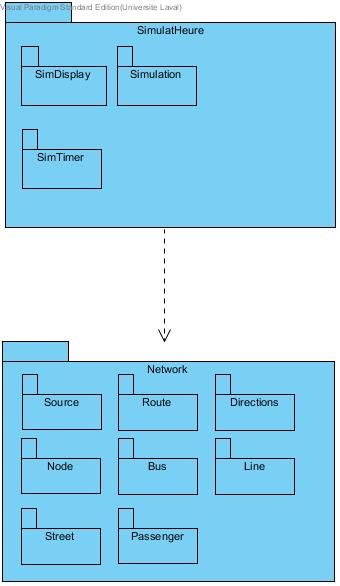
\includegraphics[scale=0.5]{fig/packageDiagram.jpg}
	\centering
	\caption{Diagramme de package de SimulatHEURE}
	\label{f:package_Diag}
\end{figure}

\section{Diagramme d'�tats}

\begin{figure}[H]
	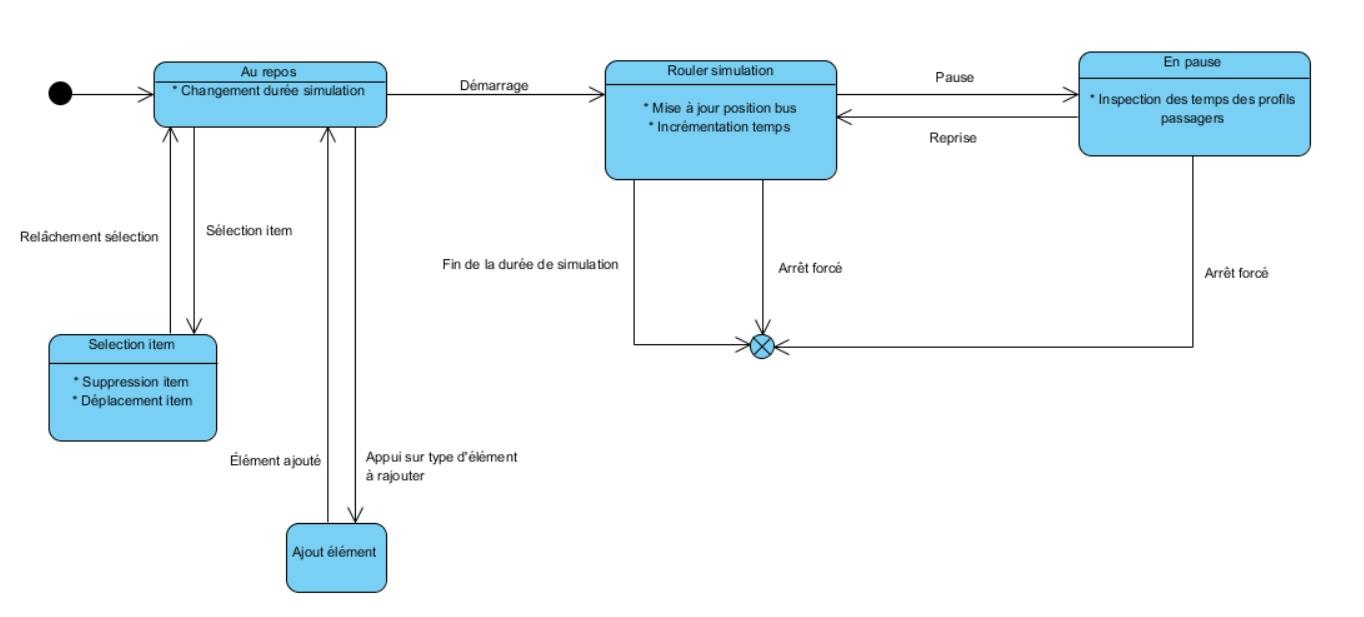
\includegraphics[scale=0.6]{fig/StateDiagram.jpg}
	\centering
	\caption{Diagramme d'�tat de SimulatHEURE}
	\label{f:state_Diag}
\end{figure}

\section{Diagramme d'activit�}

\begin{figure}[H]
	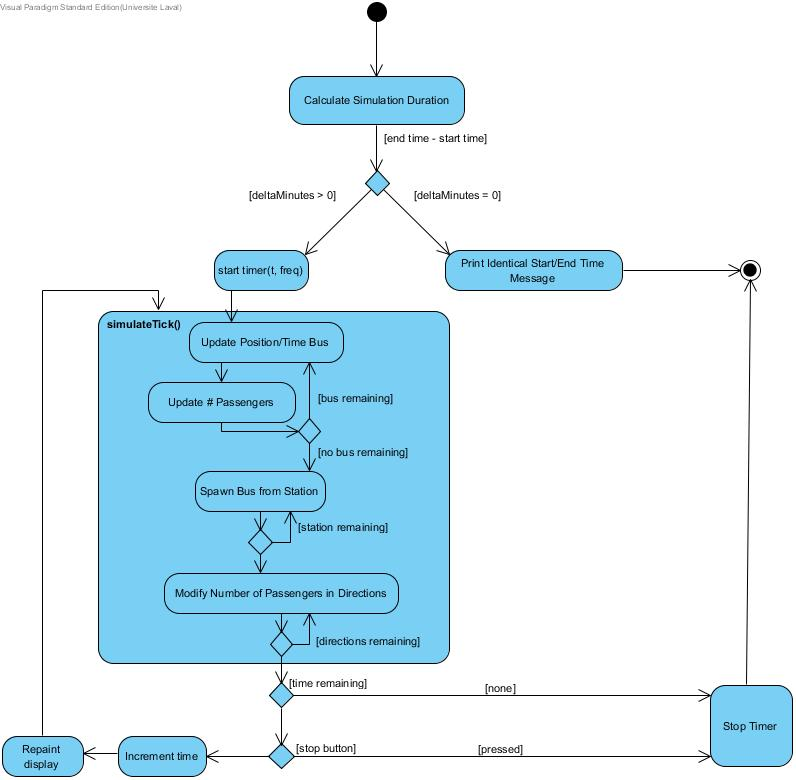
\includegraphics[scale=0.5]{fig/activityDiagram.jpg}
	\centering
	\caption{Diagramme d'activit� de SimulatHEURE}
	\label{f:activity_Diag}
\end{figure}

Lors du d�marrage de la simulation, les heures de d�part et de fin sont s�lectionn�es. Si celles-ci sont �gales, un message d'erreur est affich�, sinon la simulation d�bute. Le timer est d�marr� avec un dur�e (t) et une fr�quences (freq) afin de d�terminer la longueur d'un tick. � chaque "tick", les positions de chaque bus et la dur�e de leur trajet sont actualis�s. Dans chaque station, les bus appara�ssent � chaque station selon la fr�quence de chacune. Par la suite, pour chaque trajet, le nombre de passagers est modifi�. Si le temps actuel est �gal au temps de fin, ou si le bouton stop est appuy�, la simulation arr�te. Sinon, le temps est incr�ment�, l'affichage remis � jour et l'ex�cution continue.